\chapter{Binary Search}
\label{ch:binsearch}

\newcommand{\lecnum}{6}
%\newcommand{\lectitle}{Binary Search}
\newcommand{\lecturer}{Frank Pfenning}

\chapterTAGS{complexity, correctness, divide-and-conquer, loop-invariant, safety, search, testing}
\maketitle

\begin{preamble}
\noindent
One of the fundamental and recurring problems in computer science is
to find elements in collections, such as elements in sets.  An
important algorithm for this problem is \emph{binary search}.  We use
binary search to look for an integer in a sorted array to exemplify
it.  We started in a previous lecture by discussing \emph{linear
  search} and giving some background on the problem.  This lecture
clearly illustrates the power of \emph{order} in algorithm design: if
an array is sorted we can search through it very efficiently, much
more efficiently than when it is not ordered.

We will also once again see the importance of loop invariants in
writing correct code.  Here is a note by Jon Bentley about binary
search:
\begin{quote}\em
  I've assigned [binary search] in courses at Bell Labs and IBM.
  Professional programmers had a couple of hours to convert [its]
  description into a program in the language of their choice; a
  high-level pseudo-code was fine.  At the end of the specified time,
  almost all the programmers reported that they had correct code for
  the task.  We would then take thirty minutes to examine their code,
  which the programmers did with test cases.  In several classes and
  with over a hundred programmers, the results varied little: ninety
  percent of the programmers found bugs in their programs (and I
  wasn't always convinced of the correctness of the code in which no
  bugs were found).

  I was amazed: given ample time, only about ten percent of
  professional programmers were able to get this small program right.
  But they aren't the only ones to find this task difficult: in the
  history in Section 6.2.1 of his Sorting and Searching, Knuth points
  out that while the first binary search was published in 1946, the
  first published binary search without bugs did not appear until
  1962.

  \hfill ---Jon Bentley, \emph{Programming Pearls} (1st edition), pp.35--36
\end{quote}
I contend that what these programmers are missing is the understanding
of how to use loop invariants in composing their programs.  They help
us to make assumptions explicit and clarify the reasons \emph{why} a
particular program is correct.  Part of the magic of pre- and
post-conditions as well as loop invariants and assertions is that they
\emph{localize} reasoning.  Rather than having to look at the whole
program, or the whole function, we can focus on individual statements
tracking properties via the loop invariants and assertions.
\end{preamble}

\begin{gram}[Learning Goals]
The learning goals for this lecture are as follows:
\begin{description}
\item[Computational Thinking: ]%
  Obtaining an exponential speed-up by partitioning the problem space --- a
  prelude to a more general technique called divide-and-conquer.
\item[Algorithms and Data Structures: ]%
  Binary search.
\item[Programming: ]%
  Using loop invariants as a design tool for programs.
\end{description}
\end{gram}


\section{Binary Search}
\label{sec:binsearch:theory}
\TAGS{complexity, divide-and-conquer, search}

Can we do better than searching through the array linearly?  If you don't know
the answer already it might be surprising that, yes, we can do
\emph{significantly} better!  Perhaps almost equally surprising is that the
code is almost as short!  However, this will require the array to be
\emph{sorted}.

Before we write the code, let us describe the algorithm.  We start
searching for $x$ by examining the \emph{middle element} of the sorted
array.  If it is smaller than $x$, then $x$ must be in the upper half
of the array (if it is there at all); if it is greater than $x$, then
$x$ must be in the lower half.  Now we continue by restricting our
attention to either the upper or lower half, again finding the middle
element and proceeding as before.

We stop if we either find $x$, or if the size of the subarray
shrinks to zero, in which case $x$ cannot be in the array.

Before we write a program to implement this algorithm, let us analyze the
running time.  Assume for the moment that the size of the array is a power of
2, say $2^k$.  Each time around the loop, when we examine the middle element,
we cut the size of the subarrays we look at in half.  So before the first
iteration the size of the subarray of interest is $2^k$.  After the first
iteration (i.e., just before the second), it is of size $2^{k-1}$, then
$2^{k-2}$, etc.  After $k$ iterations it will be $2^{k-k} = 1$, so we stop
after the next iteration.  Altogether we can have at most $k+1$ iterations.
Within each iteration, we perform a constant amount of work: computing the
midpoint, and a few comparisons.  So, overall, when given a size of array $n$
we perform $c \times \log_2 n$ operations (for some constant
$c$).\footnote{In general in computer science, we are mostly interested in
  logarithm to the base $2$ so we will just write $\log n$ for log to
  the base $2$ from now on unless we are considering a different base.}

If the size $n$ is not a power of 2, then we can round $n$ up to the
next power of 2, and the reasoning above still applies.  For example,
if $n = 13$ we round it up to $16 = 2^4$.  The actual number of steps
can only be smaller than this bound, because some of the actual
subintervals may be smaller than the bound we obtained when rounding
up $n$.

The logarithm grows much more slowly than the linear function that we
obtained when analyzing linear search.  As before, suppose we double
the size of the input, $n' = 2 \times n$.  Then the number of
operations will be $c \times \log (2 \times n) = c \times (\log 2 +
\log n) = c \times (1 + \log n) = c + c \times \log n$.  So the number
of operations increases only by a constant amount $c$ when we double
the size of the input.  Considering that the largest representable
positive number in 32-bit two's complement representation is
$2^{31}-1$ (about 2 billion) binary search even for unreasonably large
arrays will only traverse the loop $31$ times!


\section{Implementing Binary Search}
\label{sec:binsearch:impl}
\TAGS{correctness, loop-invariant, safety, search}

The specification for binary search is the same as for linear search.
\begin{lstlisting}[language={[C0]C}, numbers=left]
int binsearch(int x, int[] A, int n)
//@requires 0 <= n && n <= \length(A);
//@requires is_sorted(A, 0, n);
/*@ensures (-1 == \result && !is_in(x, A, 0, n))
        || ((0 <= \result && \result < n) && A[\result] == x);
  @*/
  ;
\end{lstlisting}
We declare two variables, \lstinline'lo' and \lstinline'hi', which hold the
lower and upper end of the subinterval in the array that we are
considering.  We start with \lstinline'lo' as $0$ and \lstinline'hi' as
$n$, so the interval includes \lstinline'lo' and excludes \lstinline'hi'.
This often turns out to be a convenient choice when computing with
arrays (but see Exercise~\ref{exc:binsearch-inclusive}).

The \lstinline'for' loop from linear search becomes a \lstinline'while' loop,
exiting when the interval has size zero, that is,
\lstinline'lo == hi'.  We can easily write the first loop invariant,
relating \lstinline'lo' and \lstinline'hi' to each other and the overall
bound of the array.

\begin{lstlisting}[language={[C0]C}, numbers=left]
int binsearch(int x, int[] A, int n)
//@requires 0 <= n && n <= \length(A);
//@requires is_sorted(A, 0, n);
/*@ensures (-1 == \result && !is_in(x, A, 0, n))
        || ((0 <= \result && \result < n) && A[\result] == x);
  @*/
{
  int lo = 0;
  int hi = n;
  while (lo < hi)
  //@loop_invariant 0 <= lo && lo <= hi && hi <= n;
  {
    // ...??...
   }
  return -1;
}
\end{lstlisting}

In the body of the loop, we first compute the midpoint $\mathit{mid}$.  By
elementary arithmetic it is indeed between $\mathit{lo}$ and $\mathit{hi}$.

%  We
% assert that the midpoint is indeed between $\mathit{lo}$ and
% $\mathit{hi}$.  That assertion is easy to see, because
% $\mathit{lo}<\mathit{hi}$ (by loop condition) and therefore
% $\mathit{hi}-\mathit{lo} > 0$.  Furthermore, $\mathit{lo} +
% (\mathit{hi}-\mathit{lo}) = \mathit{hi}$, so if we divide the
% second summand by $2$ (which truncates towards $0$), we will have
% $\mathit{lo}+(\mathit{hi}-\mathit{lo})/2 < \mathit{hi}$.

Next in the loop body we check if $A[\mathit{mid}] = x$.  If so, we
have found the element and return $\mathit{mid}$.
\begin{lstlisting}[language={[C0]C}, numbers=left]
int binsearch(int x, int[] A, int n)
//@requires 0 <= n && n <= \length(A);
//@requires is_sorted(A, 0, n);
/*@ensures (-1 == \result && !is_in(x, A, 0, n))
        || ((0 <= \result && \result < n) && A[\result] == x);
  @*/
{
  int lo = 0;
  int hi = n;
  while (lo < hi)
    //@loop_invariant 0 <= lo && lo <= hi && hi <= n;
    //@loop_invariant ...??...;
    {
      int mid = lo + (hi-lo)/2;
      //@assert lo <= mid && mid < hi;
      if (A[mid] == x) return mid;
      // ...??...
    }
  return -1;
}
\end{lstlisting}

Now comes the hard part.  What is the missing part of the invariant?
The first instinct might be to say that $x$ should be in the interval
from $A[\mathit{lo}]$ to $A[\mathit{hi}]$.  But that may not
even be true when the loop is entered the first time.

Let's consider a generic situation in the form of a picture and
collect some ideas about what might be appropriate loop invariants.
Drawing diagrams to reason about an algorithm and the code that we are
trying to construct is an extremely helpful general technique.
\begin{center}
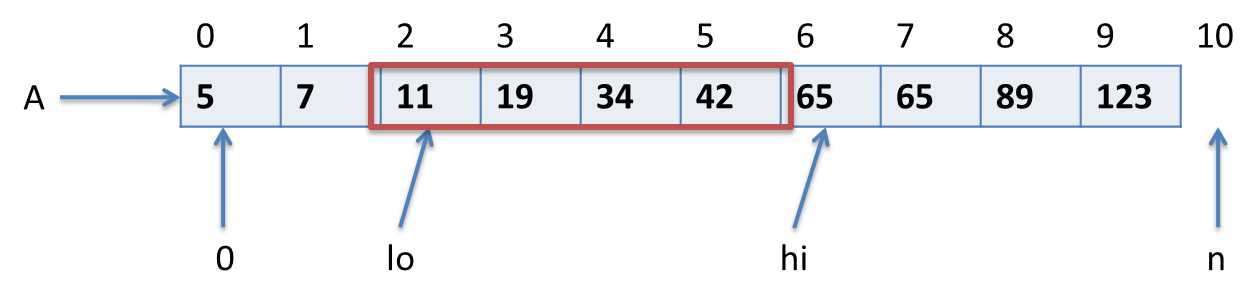
\includegraphics[width=0.85\textwidth]{img/binsearch1.png}
\end{center}

The red box around elements 2 through 5 marks the segment of the array still
under consideration.  This means we have \emph{ruled out} everything to the
right of (and including) $\mathit{hi}$ and to the left of (and not including)
$\mathit{lo}$.  Everything to the left is ruled out, because those values have
been recognized to be strictly less than $x$, while the ones on the right are
known to be strictly greater than $x$, while the middle is still unexplored.

We can depict this as follows:
\begin{center}
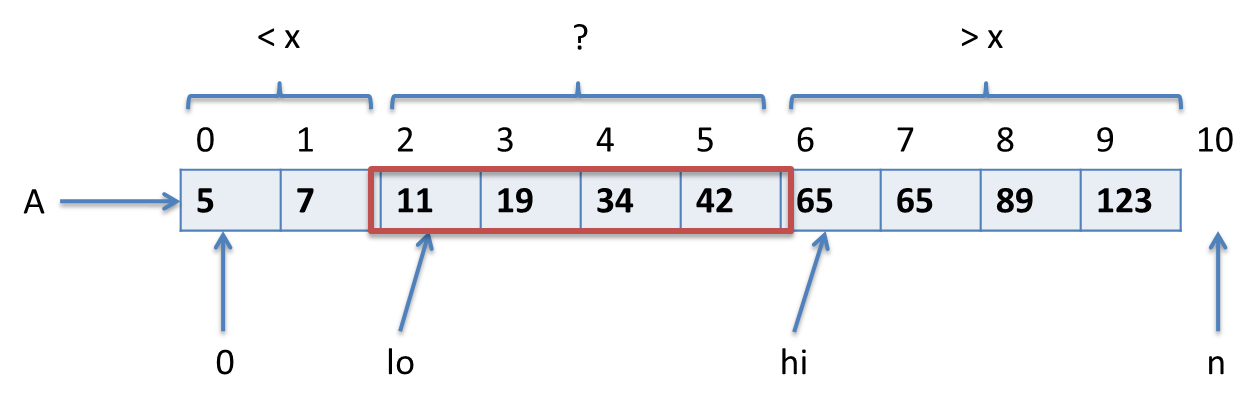
\includegraphics[width=0.85\textwidth]{img/binsearch2.png}
\end{center}

We can summarize this by stating that $A[\mathit{lo}-1] < x$ and
$A[\mathit{hi}] > x$.  This implies that $x$ cannot be in the
segments $A\lbrack 0{..}\mathit{lo})$ and $A\lbrack \mathit{hi}{..}n)$ because the
array is sorted (so all array elements to the left of
$A[\mathit{lo}-1]$ will also be less than $x$ and all array
elements to the right of $A[\mathit{hi}]$ will also be greater than
$x$).  For an alternative, see Exercise~\ref{exc:binsearch-isin}.

We can postulate these as invariants in the code.

\clearpage
\begin{lstlisting}[language={[C0]C}, numbers=left]
int binsearch(int x, int[] A, int n)
//@requires 0 <= n && n <= \length(A);
//@requires is_sorted(A, 0, n);
/*@ensures (-1 == \result && !is_in(x, A, 0, n))
       || ((0 <= \result && \result < n) && A[\result] == x);
  @*/
{
  int lo = 0;
  int hi = n;
  while (lo < hi)
    //@loop_invariant 0 <= lo && lo <= hi && hi <= n;
    //@loop_invariant A[lo-1] < x;
    //@loop_invariant A[hi] > x;
    {
      int mid = lo + (hi-lo)/2;
      if (A[mid] == x) return mid;
      // ...??...
   }
  return -1;
}
\end{lstlisting}

Now a very powerful programming instinct should tell you something is
fishy.  Can you spot the problem with the new invariants even
before writing any more code in the body of the loop?

\clearpage
\begin{quote}\em
  Whenever you access an element of an array, you must have
  good reason to know that the access will be in bounds!
\end{quote}

In the code we blithely wrote $A[\mathit{lo}-1]$ and
$A[\mathit{hi}]$ because they were in the middle of the
array in our diagram.  But initially (and potentially
through many iterations) this may not be the case.
Fortunately, it is easy to fix, following what we did
for linear search.  Consider the following picture when
we start the search.
\begin{center}
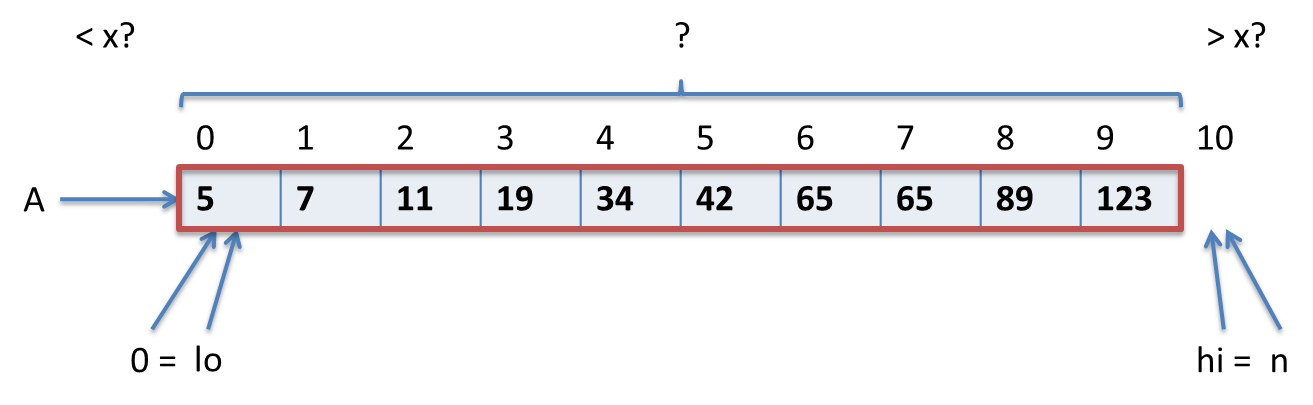
\includegraphics[width=0.99\textwidth]{img/binsearch3.png}
\end{center}

In this case all elements of the array have to be considered
candidates.  All elements strictly to the left of $0$ (of which there
are none) and to the right of $n$ (of which there are none) have been
ruled out.  As in linear search, we can add this to the our invariant
using disjunction.
% , which uses short-circuiting evaluation that the
% array will not be accessed if the access were out of bounds.

\begin{lstlisting}[language={[C0]C}, numbers=left]
int binsearch(int x, int[] A, int n)
//@requires 0 <= n && n <= \length(A);
//@requires is_sorted(A, 0, n);
/*@ensures (-1 == \result && !is_in(x, A, 0, n))
       || ((0 <= \result && \result < n) && A[\result] == x);
  @*/
{
  int lo = 0;
  int hi = n;
  while (lo < hi)
    //@loop_invariant 0 <= lo && lo <= hi && hi <= n;
    //@loop_invariant (lo == 0 || A[lo-1] < x);
    //@loop_invariant (hi == n || A[hi] > x);
    {
      int mid = lo + (hi-lo)/2;
      if (A[mid] == x) return mid;
      // ...??...
   }
  return -1;
}
\end{lstlisting}

At this point, let's check if the loop invariant is strong enough
to imply the post-condition of the function.  If we return from inside
the loop because $A[\mathit{mid}] = x$ we return $\mathit{mid}$,
so \lstinline'A[\result] == x' as required.

If we exit the loop because $\mathit{lo} < \mathit{hi}$ is
false, we know $\mathit{lo} = \mathit{hi}$, by the first
loop invariant.  Now we have to distinguish some cases.
\begin{enumerate}
\item If $A[\mathit{lo}-1] < x$ and $x < A[\mathit{hi}]$, then
  $x < A[\mathit{lo}]$ (since $\mathit{lo} = \mathit{hi}$).
  Because the array is sorted, $x$ cannot be in it.
\item If $\mathit{lo} = 0$, then $\mathit{hi} = 0$.
  By the third loop invariant, then either $n = 0$ (and so the array has
  no elements and we must return $-1$), or $A[\mathit{hi}] =
  A[\mathit{lo}] = A[0] > x$.  Because $A$ is sorted, $x$ cannot
  be in $A$ if its first element is already strictly greater than $x$.
\item If $\mathit{hi} = n$, then $\mathit{lo} = n$.
  By the second loop invariant, then either $n = 0$ (and so we must return
  $-1$), or $A[n-1] = A[\mathit{hi}-1] = A[\mathit{lo}-1] < x$.
  Because $A$ is sorted, $x$ cannot be in $A$ if its last element
  is already strictly less than $x$.
\end{enumerate}

Notice that we could verify all this without even knowing the complete
program!  As long as we can finish the loop to preserve the invariant
and terminate, we will have a correct implementation!  This would
again be a good point for you to interrupt your reading and to try to
complete the loop, reasoning from the invariant.

We have already tested if $A[\mathit{mid}] = x$.  If not, then
$A[\mathit{mid}]$ must be less or greater than $x$.  If it is less,
then we can keep the upper end of the interval as is, and set the
lower end to $\mathit{mid}+1$.  Now $A[\mathit{lo}-1] < x$ (because
$A[\mathit{mid}] < x$ and $\mathit{lo} = \mathit{mid}+1$), and the
condition on the upper end remains unchanged.

If $A[\mathit{mid}] > x$ we can set $\mathit{hi}$ to $\mathit{mid}$
and keep $\mathit{lo}$ the same.  We do not need to test this last
condition, because the fact that the tests $A[\mathit{mid}] = x$ and
$A[\mathit{mid}] < x$ both failed implies that $A[\mathit{mid}] > x$.
We note this in an assertion.

\clearpage

\begin{lstlisting}[language={[C0]C}, numbers=left]
int binsearch(int x, int[] A, int n)
//@requires 0 <= n && n <= \length(A);
//@requires is_sorted(A, 0, n);
/*@ensures (-1 == \result && !is_in(x, A, 0, n))
       || ((0 <= \result && \result < n) && A[\result] == x);
 @*/
{ int lo = 0;
  int hi = n;
  while (lo < hi)
    //@loop_invariant 0 <= lo && lo <= hi && hi <= n;
    //@loop_invariant (lo == 0 || A[lo-1] < x);
    //@loop_invariant (hi == n || A[hi] > x);
    {
      int mid = lo + (hi-lo)/2;
      //@assert lo <= mid && mid < hi;
      if (A[mid] == x) return mid;
      else if (A[mid] < x) lo = mid+1;
      else /*@assert(A[mid] > x);@*/
        hi = mid;
    }
  return -1;
}
\end{lstlisting}

\clearpage
Let's set up the proof of the loop invariants more schematically.
\begin{description}
\item[Init: ]%
  When the loop is first reached, we have $\mathit{lo} = 0$ and $\mathit{hi} =
  n$, so the first loop invariant follows from the precondition to the
  function.  Furthermore, the first disjunct in loop invariants two
  (\lstinline'lo == 0') and three (\lstinline'hi == n') is satisfied.
\item[Preservation: ]%
  Assume the loop invariants are satisfied and we enter the loop:
  $$
  \begin{array}{ll}
     0 \leq \mathit{lo} \leq \mathit{hi} \leq n           & \text{(Inv 1)}
  \\ (\mathit{lo} = 0\; \text{or}\; A[\mathit{lo}-1] < x) & \text{(Inv 2)}
  \\ (\mathit{hi} = n\; \text{or}\; A[\mathit{hi}] > x)   & \text{(Inv 3)}
  \\ \mathit{lo} < \mathit{hi}                            & \text{(loop condition)}
  \end{array}
  $$
  We compute $\mathit{mid} = \mathit{lo} + \lfloor (\mathit{hi}-\mathit{lo})/2
  \rfloor$.  Now we distinguish three cases:
  \begin{description}
  \item[{$A[\mathit{mid}] = x$}: ]%
    In that case we exit the function, so we don't need to show preservation.
    We do have to show the post-condition, but we already considered this
    earlier in the lecture.
  \item[{$A[\mathit{mid}] < x$}: ]%
    Then
    $$
    \begin{array}{l}
       \mathit{lo}' = \mathit{mid}+1
    \\ \mathit{hi}' = \mathit{hi}
    \end{array}
    $$
    The first loop invariant $0 \leq \mathit{lo}' \leq \mathit{hi}' \leq n$
    follows from the formula for $\mathit{mid}$, our assumptions, and
    elementary arithmetic.

    For the second loop invariant, we calculate:
    $$
    \begin{array}{lcll}
       A[\mathit{lo}'-1] &=& A[(\mathit{mid}+1)-1]
     & \text{since } \mathit{lo}' = \mathit{mid}+1
    \\                   &=& A[\mathit{mid}]
     & \text{by arithmetic}
    \\                   &<& x
     & \text{this case } A[\mathit{mid}] < x
    \end{array}
    $$
    The third loop invariant is preserved, since $\mathit{hi}' =
    \mathit{hi}$.
  \item[{$A[\mathit{mid}] > x$}: ]%
    Then
    $$
    \begin{array}{l}
       \mathit{lo}' = \mathit{lo}
    \\ \mathit{hi}' = \mathit{mid}
    \end{array}
    $$
    Again, by elementary arithmetic, $0 \leq \mathit{lo}' \leq \mathit{hi}' \leq n$.

    The second loop invariant is preserved since $\mathit{lo}' =
    \mathit{lo}$.

    For the third loop invariant, we calculate
    $$
    \begin{array}{lcll}
       A[\mathit{hi}'] &=& A[\mathit{mid}]
     & \text{since } \mathit{hi}' = \mathit{mid}
    \\                 &>& x
     & \text{since we are in the case } A[\mathit{mid}] > x
    \end{array}
    $$
  \end{description}
\end{description}


\section{Termination}
\label{sec:binsearch:term}
\TAGS{correctness, search}

Does this function terminate?  If the loop body executes, that is,
$\mathit{lo} < \mathit{hi}$, then the interval from
$\mathit{lo}$ to $\mathit{hi}$ is non-empty.  Moreover, the
intervals from $\mathit{lo}$ to $\mathit{mid}$ and from
$\mathit{mid}+1$ to $\mathit{hi}$ are both strictly smaller than
the original interval.  Unless we find the element, the difference
between $\mathit{hi}$ and $\mathit{lo}$ must eventually become
$0$ and we exit the loop.


\section{One More Observation}
\label{sec:binsearch:edge}
\TAGS{correctness}

You might be tempted to calculate the midpoint with
\begin{lstlisting}[language={[C0]C}, numbers=left, firstnumber=13]
int mid = (lo + hi)/2;
\end{lstlisting}
but that is in fact incorrect.  Consider this change and
try to find out why this would introduce a bug.

\clearpage

Were you able to see it?  It's subtle, but somewhat related to other problems
we had.  When we compute \lstinline'(lo + hi)/2;' we could actually have an
overflow, if $\mathit{lo} + \mathit{hi} > 2^{31}-1$.  This is somewhat
unlikely in practice, since $2^{31} = 2G$, about 2 billion, so the array would
have to have at least 1 billion elements.  This is not impossible, and, in
fact, a bug like this in the Java libraries\footnote{See Joshua Bloch's \href{http://googleresearch.blogspot.com/2006/06/extra-extra-read-all-about-it-nearly.html}{Extra, Extra} blog entry.} was actually exposed. %

Fortunately, the fix is simple: because $\mathit{lo} < \mathit{hi}$, we know
that $\mathit{hi} - \mathit{lo} > 0$ and represents the size of the interval.
So we can divide that in half and add it to the lower end of the interval to
get its midpoint.
\begin{lstlisting}[language={[C0]C}, numbers=left, firstnumber=13]
int mid = lo + (hi-lo)/2;   // as shown in binary search
//@assert lo <= mid && mid < hi;
\end{lstlisting}
Let us convince ourselves why the assert is correct.  The division by two will
round to zero, \emph{down} to 0 here, because $\mathit{hi} - \mathit{lo} > 0$.
Thus, \(0 \leq (\mathit{hi}-\mathit{lo})/2 < \mathit{hi}-\mathit{lo}\),
because dividing a positive number by two will make it strictly smaller.
Hence,
$$
\mathit{mid = lo + (hi-lo)}/2 < \mathit{lo + (hi-lo) = hi}
$$
Since dividing positive numbers by two will still result in a non-negative
number, the first part of the assert is correct as well.
$$
\mathit{mid = lo + (hi-lo)}/2 \geq \mathit{lo + 0 = lo}
$$

Other operations in this binary search take place on quantities bounded from
above by the \lstinline'int' $n$ and thus cannot overflow.


Why did we choose to look at the middle element and not another element at
all?  Because, whatever the outcome of our comparison to that middle element
may be, we maximize how much we have learned about the contents of the array
by doing this one comparison. If we find the element, we are happy because we
are done. If the middle element is smaller than what we are looking for,
however, we are happy as well, because we have just learned that the lower
half of the array has become irrelevant. Similarly, if the middle element is
bigger, then we have made substantial progress by learning that we never need
to look at the upper half of the array anymore.  There are other choices,
however, where binary search will also still work in essentially the same way.


\section{Some Measurements}
\label{sec:binsearch:empirical}
\TAGS{complexity, testing}

Algorithm design is an interesting mix of mathematics and an experimental
science.  Our analysis above, albeit somewhat preliminary in nature, allow us
to make some predictions of running times of our implementations.  We start
with linear search.  We first set up a file to do some experiments.  We assume
we have already tested our functions for correctness, so only timing is at
stake.  See the file \lstinline'search-time.c0' in the code directory for this
lecture.  We compile this file, together with our implementation from this
lecture, with the \lstinline'cc0' command below.  We can get an overall
end-to-end timing with the Unix \lstinline'time' command.  Note that we do not
use the \lstinline'-d' flag, since that would dynamically check contracts and
completely throw off our timings.

\begin{lstlisting}[language={[coin]C}]
% cc0 find.c0 find-time.c0
% time ./a.out
\end{lstlisting}
When running linear search 2000 times (1000 times with $x$ in the array,
and 1000 times with random $x$) on $2^{18}$ elements (256 K elements)
we get the following answer
\begin{lstlisting}[language={[coin]C}]
Timing 1000 times with 2^18 elements
0
4.602u 0.015s 0:04.63 99.5%	0+0k 0+0io 0pf+0w
\end{lstlisting}
which indicates \lstinline'4.602' seconds of user time.

Running linear search 2000 times on random arrays of size
$2^{18}$, $2^{19}$ and $2^{20}$ we get the timings on our
MacBook Pro
$$
\begin{array}{cc}
   \text{array size} & \text{time (secs)}
\\            2^{18} & 4.602
\\            2^{19} & 9.027
\\            2^{20} & 19.239
\end{array}
$$
The running times are fairly close to doubling consistently.  Due to
memory locality effects and other overheads, for larger arrays we
would expect larger numbers.

Running the same experiments with binary search we get
$$
\begin{array}{cc}
  \text{array size} & \text{time (secs)}
\\           2^{18} & 0.020
\\           2^{19} & 0.039
\\           2^{20} & 0.077
\end{array}
$$
which is much, much faster but looks suspiciously linear
as well.

Reconsidering the code we see that the time might increase linearly
because we actually must iterate over the whole array in order to
initialize it with random elements!

We comment out the testing code to measure only the initialization
time, and we see that for $2^{20}$ elements we measure $0.072$
seconds, as compared to $0.077$ which is insignificant.
Effectively, we have been measuring the time to set up the random
array, rather than to find elements in it with binary search!

This is a vivid illustration of the power of divide-and-conquer.
Logarithmic running time for algorithms grow very slowly, a crucial
difference to linear-time algorithms when the data sizes become large.

\clearpage
\section{Exercises}

\begin{exercise}
  \label{exc:binsearch-inclusive} Rewrite the binary search function so
  that both lower and upper bounds of the interval are
  \emph{inclusive}.  Make sure to rewrite the loop invariants and the
  loop body appropriately, and prove the correctness of the new
  loop invariants.  Also explicitly prove termination by giving a
  measure that strictly decreases each time around the loop and is
  bounded from below.
\end{exercise}

\begin{exercise}
  \label{exc:binsearch-isin}
  Rewrite the invariants of the binary
  search function to use \lstinline'is_in(x, A, l, u)' which returns true
  if and only if there is an $i$ such that $x = A[i]$ for $l \leq i <
  u$.  $\m{is\_in}$ assumes that $0 \leq l \leq u \leq n$ where $n$ is
  the length of the array.

  Then prove the new loop invariants, and verify that they are strong
  enough to imply the function's post-condition.
\end{exercise}

\begin{exercise}
  Binary search as presented here may not find the leftmost
  occurrence of $x$ in the array in case the occurrences are
  not unique.  Given an example demonstrating this.

  Now change the binary search function and its loop invariants so
  that it will always find the leftmost occurrence of $x$ in the given
  array (if it is actually in the array, $-1$ as before if it is not).

  Prove the loop invariants and the post-conditions for this new
  version, and verify termination.
\end{exercise}

\begin{exercise}
  If you were to replace the midpoint computation by
\begin{lstlisting}[language={[C0]C}]
int mid = (lo + hi)/2;
\end{lstlisting}
  then which part of the contract will alert you to a flaw in your thinking?
  Why? Give an example showing how the contracts can fail in that case.
\end{exercise}

\begin{exercise}
  In lecture, we used design-by-invariant to construct the loop body
  implementation from the loop invariant that we have identified before.
  We could also have maintained the loop invariant by replacing the whole
  loop body just with
  \begin{lstlisting}[language={[C0]C}]
    // .... loop_invariant elided ....
    {
      lo = lo;
      hi = hi;
    }
  \end{lstlisting}
  Prove the loop invariants for this loop body.
  What is wrong with this choice? Which part of our proofs fail, thereby
  indicating why this loop body would not implement binary search correctly?
\end{exercise}

% \clearpage
% \bibliographystyle{alpha}
% \bibliography{modal}

% \cleardoublepage
